\graphicspath{ {imgs/} }
\documentclass[../Thesis.tex]{subfiles}
\begin{document}
\chapter{General Theory}
\section{Basic Assumptions and Setup}
A test is set up with at least two buckets and a sampling rate that determines what percentage of all possible users should participate in the testing. If for a new user was decided that she takes part in the test the next part is assigning her to a bucket. Later in this chapter different mechanisms for this step will be discussed and evaluated. Now certain actions of the users are recorded.

 One is generating actions with a probability $q1$ the other generates them with a probability $q2$. The prior distribution for all $q$ is a Beta distribution, which is a convenient choice because it is a prior distribution for binomial proportions (the Beta distribution is the conjugate family for the binomial likelihood). We also assume no prior knowledge when creating the test case (uninformative prior $Beta(1,1)$). $N1$ customers get assigned to Bucket 1 and $N2$ to Bucket 2. They generate $k1$ and $k2$ actions. The posterior distributions for each individual case is:
\begin{align*}
q = f(k|N) &\propto f(N|k)f(k)\\
q1 = Beta(k1+\alpha,N1-k1+\beta) & = \frac{x^{k1+\alpha-1}(1-x)^{N1-k1+\beta -1}}{B(k1+\alpha,N1-k1+\beta)} \\
q2 = Beta(k2+\alpha,N2-k2+\beta) & = \frac{x^{k2+\alpha-1}(1-x)^{N2-k2+\beta -1}}{B(k2+\alpha,N2-k2+\beta)}
\end{align*}
So each new assignment and each new event would directly alter the distributions parameters.\textit{ Questions: What is with returning users? Or users with a high action rate? Is every user a new one?}
What is the posterior for $P(q1>q2 | k1,N1,k,2,N2)$ - that Bucket 1 performs better than Bucket 2 given the collected data? There are in principal two different ways to get an answer.
\begin{figure}[h]
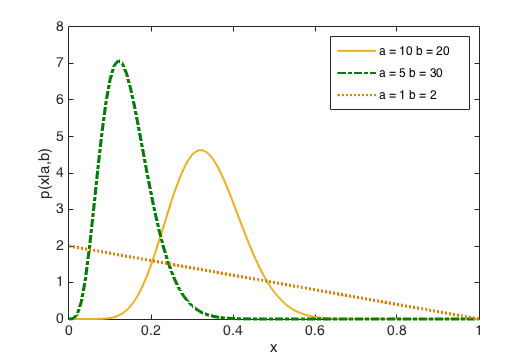
\includegraphics[scale=0.5]{BetaDists}
\centering
\title{Different Beta Distributions}
\end{figure}

\section{Best Bucket}
Finding the best Bucket among the other test scenarios can be achieved in several ways. It follows a set of methods. Each will be explained first for the simple case with two Buckets and then expanded to the general setting with n different cases.
\subsection{Analytic}
In general for two random variables $X,Y$ with corresponding probability density function $f_X,f_Y$ and cumulative density function $F_X,F_Y$ it holds: 
\begin{align*}
P(X \geq Y ) &= \iint_{[x>y]} f_X(x)f_Y(y) \,dy\,dx \\
					&= \iint_{-\infty}^{x} f_X(x)f_Y(y) \,dy\,dx \\
					&= \int_{-\infty}^{\infty}f_X(x)F_Y(x)\,dx
\end{align*}
In the paper "Numerical Computation of Stochastic Inequality Probabilities" the author John D. Cook uses symmetries of the distribution to arrive at a set of equations that can be used to calculate the problem recursively.

\begin{align*}
g(k1,N1,k2,N2) &= P(X>Y) \\
h(k1,N1,k2,N2) &= \frac{B(k1+k2,N1+N2)}{B(k1,N1)B(k2,N2)}
\end{align*}
From that one could calculate a base case for a small sample and then continue with:
\begin{align*}
g(k1 + 1,N1,k2,N2) &= g(k1,N1,k2,N2) + h(k1,N1,k2,N2)/k1 \\
g(k1,N1 + 1,k2,N2) &= g(k1,N1,k2,N2) - h(k1,N1,k2,N2)/N1 \\
g(k1,N1,k2 + 1,N2) &= g(k1,N1,k2,N2) - h(k1,N1,k2,N2)/k2 \\
g(k1,N1,k2,N2 + 1) &= g(k1,N1,k2,N2) + h(k1,N1,k2,N2)/N2 \\
\end{align*}


\subsection{Approximation}
For \textit{sufficient large} samples one could again approximate the Beta Distribution with a normal distribution. This means that the following equation should be fulfilled for $B(k,N)$:
\begin{align*}
\frac{k + 1}{k - 1}\approx 0,
\frac{N + 1}{N - 1}\approx 0
\end{align*}
The Gaussian Distribution to a given Beta Distribution has the following shape:
\begin{align*}
B(k,N)\approx N\left(\frac{k}{k+N},\sqrt{\frac{kN}{(k+N)^2(k+N+1)}} \right)
\end{align*}
The inequality for this case then could be solved by:
\begin{align*}
P(X>Y)	&= P(0 > Y - X) \\
			&= P(0 > \mu_Y - \mu_X + (\sigma_X^2 + \sigma_Y^2)^{\frac{1}{2}}Z) \\
			&= P\left(Z < \frac{\mu_X - \mu_Y}{(\sigma_X^2 + \sigma_Y^2)^{\frac{1}{2}}}\right) \\
			&= \Phi\left(\frac{\mu_X - \mu_Y}{(\sigma_X^2 + \sigma_Y^2)^{\frac{1}{2}}}\right)
\end{align*}
I am not sure if this is really a smart way to do it but what would be maybe interesting is finding out which of the possibilities is the fastest for growing $N$.

\subsection{Sampling}
One could also sample from the different distributions and take the mean of the of the samples to determine the best distribution. The mean of a Beta distribution $B(k,N)$ is given by:
\begin{align*}
E[X] = \frac{k}{k+N}
\end{align*}
Open question here: how exactly is the sample size related to the accuracy of the estimate?

\subsection{n Buckets}
The generalization would again depend on the chosen method to evaluate the inequality.
\subsubsection{Analytic}
I found examples for 3 Beta distributed random variables. But basically any formula would calculate the probability that one variable is greater than the others which results in $n-1$ equations to solve the problem for $n$ buckets. The same number of equations would occur if we would compute the inequality pairwise with the already presented formula.

\subsubsection{Sampling}
Additional Buckets would not change the underlying computation but would result in additional draws and new means to compare. 

\section{Best Assignment}
It is not obvious what the best strategy is to assign a new user to a specific bucket. I will try to compare several intuitive approaches in this section. Interesting cases for the different strategies are: How fast does each strategy converge? What happens if there is no clear winner?
\subsection{Uniform}
\subsection{Random}
\subsection{Entropy}
The best assignment for a not yet tracked user would be a bucket that minimizes the entropy over the different buckets. The entropy of a Beta Distribution is given by:
\begin{align*}
h(q) 	&= E[-ln(f(x;k,N))] \\
		&= \int_{0}^{1} -f(x;k,N)ln(f(x;k,N))\,dx \\
		&= ln(B(k,N)) - (k-1) \psi(k) - (N-1) \psi(N) + (k+N-2) \psi(k+N)
\end{align*}
Where $\psi$ is the Digamma function. One could calculate the difference from $h(q_x)$ to $h(q_x')$ where $x \in {1...n}$ number of Buckets and $q_x'$ represents the distribution with the newly assigned user and assign the user the bucket where $max(|h(q_x)-h(q_x')|)$.

\end{document}